\textbf{\LARGE osn 18. Операционные системы. Процессы, взаимодействие процессов, разделяемые ресурсы, синхронизация взаимодействующих процессов, взаимное исключение. Программирование взаимодействующих процессов с использованием средств ОС UNIX (сигналы, неименованные каналы, IPC).}

\textbf{Операционная система} --- комплекс программ, используемых для управления ресурсами компьютера и предоставления интерфейса пользователю.
В понятие управление ресурсами входит \textit{выделение} ресурсов для программ (например, памяти и процессорного времени),
\textit{защита} от доступа программ к ресурсам, которыми они не владеют, а также
\textit{абстрагирование} от оборудования, например, предоставление общего интерфейса для похожих типов устройств
(общий файловый интерфейс для всех дисков) или реализация виртуальных ресурсов (увеличение эффективного объема памяти за счет файла подкачки).

\textbf{Физические ресурсы (устройства)} -- компоненты аппаратуры компьютера, используемые на программных уровнях ВС или оказывающие влияние на функционирование всей ВС. Совокупность физических ресурсов составляет аппаратный уровень вычислительной системы.

\textbf{Логические, или виртуальные ресурсы (устройства) ВС} -- устройство/ресурс, некоторые эксплуатационные характеристики которого (возможно все) реализованы программным образом.

\textbf{Состав ОС:} 
\begin{itemize}
    \item ядро ОС - резидентная часть ОС, реализующая некоторую базовую функциональность ОС и работающая в режиме супервизора;
    \item динамически подгружаемые драйверы физических и виртуальных устройств. под динамически подгружаемыми понимается то, что в зависимости от ситуации состав этих драйверов при инсталяции и загрузке системы может меняться;
    \item интерфейсы системных вызовов.
\end{itemize} 

\textbf{Типы ОС:} 

- Пакетные ос  - система, критерием эффективности которой является максимальная загрузка ЦП. Время работы процессора/время работы исполнения пользовательских программ ~ 1. Пакет программ - совокупность программ которые системе необходимо обработать. Переключение процессов происходит по 1 из трех причин: зацикливание процесса, завершение процесса, обращение к внешнему устройству. 

- ОС разделения времени - модель, представляющая собой развитие пакетных систем. Дополнительная характеристика - квант процессорного времени - некоторый фиксированный ос промежуток времени работы процессора. + причина по смене исполняемого процесса - исчерпание кванта времени. 

- ОС реального времени - системы, ориентированные на обработку некоторого фиксированного набора событий, при возникновении любого из которых гарантируется обработка этого события за некоторый промежуток времени, не превосходящий определенного предельного значения. 

- Сетевые ОС - ос, обеспечивающая функционирование и взаимодействие вычислительной системы в пределах сети. 

- Распределенная система - система, функционирующая на многопроцессорном/многомашинном комплексе, в котором на каждом из узлов функционирует отдельное ядро, а сама система обеспечивает реализацию распределенных возможностей ОС. 

Под \textbf{процессом} понимается совокупность машинных команд и данных, обрабатываемая в вычислительной системе и обладающая правами на владение некоторым набором ресурсов ВС. \textbf{Процесс (полновесный)} - объект планирования и выполняется внутри защищённой области памяти. \textbf{Легковесные процессы} - могут активироваться внутри полновесного процесса, могут быть объектами планирования, и при этом они могут функционировать внутри общей (т.е. незащищённой от других нитей) области памяти. Понятие процесса включает в себя следующее:исполняемый код, собственное адресное пространство, представляющее собой множество виртуальных адресов, которые может использовать процесс, ресурсы сиcтемы, которые назначены процессу ос, хотя бы одну выполняемую нить. 
\textbf{Системный вызов} - средство ос, предоставляемое пользователям (процессам), посредством которого процессы могут обращаться к ядру ос за выполнением тех или иных функций.
\textbf{Процесс} - объект, порожденный системным вызовом \textbf{fork}. 
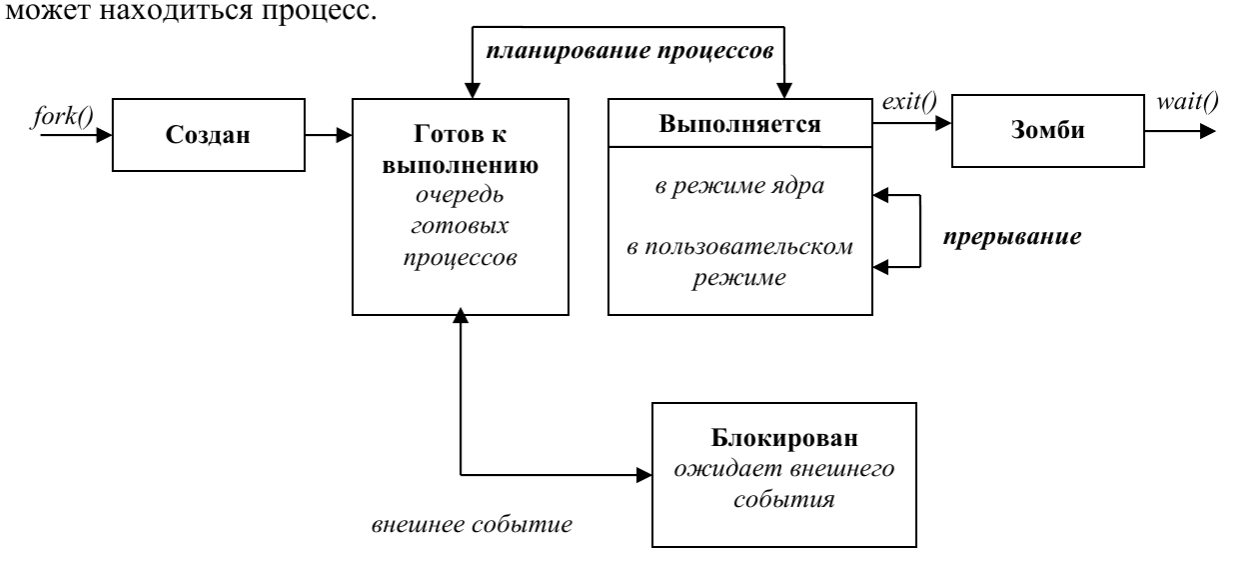
\includegraphics[scale=0.27]{pics/life_cycle.png}

Будем говорить, что процессы называются \textbf{параллельными}, если их выполнение хотя бы частично перекрывается по времени.
Совместное использование ресурса ВС двумя и более параллельными процессами, когда каждый некоторое время владеет этим ресурсом, называется \textbf{разделением ресурса.} Ситуация, когда процессы конкурируют за разделяемый ресурс, называются \textbf{гонкой процессов}. \textbf{Критический ресурс} - разделяемый ресурс, который в каждый момент времени доступен только одному из взаимодействующих процессов.  

\textbf{Пример.} Имеется разделяемый ресурс \textit{in} и два процесса. В некоторый момент времени процесс $A$ присвоил переменной \textit{in} значение $X$. Затем в некоторый момент процесс $B$ присвоил значение $Y$ этой же переменной \textit{in}. Далее оба процесса читают эту переменную, и в обоих случаях процессы прочтут значение $Y$ . То есть символ, считанный процессом $A$, был потерян, а символ, считанный процессом $B$, был выведен дважды. Результат выполнения процессов здесь зависит от того, в какой момент осуществляется переключение процессов, и от того, какой конкретно процесс будет выбран следующим для выполнения.

\textbf{Взаимное исключение} - способ работы с разделяемым ресурсом, при котором когда один из процессов работает с разделяемым ресурсом, все остальные не могут иметь к нему доступ.

\textbf{Блокировка} - доступ к разделяемому ресурсу одного из взаимодействующих процессов не обеспечивается из-за активности более приоритетных.

\textbf{Тупик} - взаимоблокировка.

\textbf{Семафоры Дейкстры}

Имеется специальный тип данных --- \textit{семафор}. Переменные типа семафор могут принимать целочисленные значения. Определены атомарные операции: опустить семафор \textit{down(S)} (или \textit{P(S)}) и поднять семафор \textit{up(S)} (или \textit{V(S)}).

Операция \textit{down(S)} проверяет значение семафора \textit{S} и, если оно больше нуля, то уменьшает его на 1. Если же это не так, процесс блокируется, причем связанная с заблокированным процессом операция down считается незавершенной.

Операция \textit{up(S)} увеличивает значение семафора на 1. При этом если в системе присутствуют процессы, блокированные ранее при выполнении \textit{down} на этом семафоре, то один из них разблокируется и завершает выполнение операции \textit{down}, т.е. вновь уменьшает значение семафора. Выбор процесса для разблокирования никак не оговаривается. Используется для предотвращения тупика. 

\textbf{Монитор} - это языковая конструкция с централизованным управлением (в отличие от семафоров, которые не обладают централизацией).
\begin{enumerate}
    \item Cтруктуры данных монитора доступны только через обращения к процедурам или функциям этого монитора (т.е. монитор представляет собой некоторый аналог объекта в объектно-ориентированных языках и реализует инкапсуляцию данных);
    \item процесс занимает (или входит в) монитор, если он вызывает одну из процедур или функций монитора;
    \item В каждый момент времени внутри монитора может находиться не более одного процесса.
\end{enumerate}

\textbf{Механизм передачи сообщений} основан на двух функциональных примитивах: \textit{send} и \textit{receive}. Их можно разделить по трем характеристикам: модель синхронизации (операции посылки/приема сообщений могут быть блокирующими и неблокирующими), адресация (прямая (конкретный адрес) или косвенная (сообщение бросается в общий пул)) и формат сообщения.   

\textbf{Сигналы} --- средство оказания воздействия одним процессом на другой процесс (одним из них может быть ОС). Используются непосредственные имена процессов. Асинхронное взаимодействие (момент прихода сигнала заранее неизвестен). Действия при получении: обработка по умолчанию(процесс завершается с кодом сигнала), специальная обработка(вызывается спец ф-я), игнорирование. Порядок реагирования не определен. Чтобы установить реакцию процесса на приходящий сигнал, используется системный вызов \textit{signal()}.

\textbf{Неименованый канал} (англ. pipe) - это объект, позволяющий реализовать односторонний канал между двумя процессами. Создается вызовом \textit{pipe()}, который возвращает два файловых дескриптора, один на чтение, другой на запись. Один процесс пишет в файловый дескриптор на запись, другой читает из файлового дескриптора на чтение. При этом реального файла в файловой системе нет.

Предельный размер канала декларируется параметрами настройки ОС. Для создания -- системный вызов $pipe()$. К неименованному каналу невозможен доступ по имени, существует в системе, пока существуют процессы, его использующие. Предназначен для синхронизации и организации взаимодействия родственных процессов.

\textbf{IPC} (Inter-Process Communication) предоставляет взаимодействующим процессам общие (разделяемые) ресурсы.
Например, SytemV IPC предоставляет следующие типы разделяемых ресурсов:
\begin{itemize}
    \item \textbf{Очередь сообщений} - это разделяемый ресурс, позволяющий организовывать очереди сообщений: один процесс может в эту очередь положить сообщение, а другой процесс - прочитать его.
    \item \textbf{Массив семафоров} - ресурс, представляющий собой массив из N элементов, где N задается при создании данного ресурса, и каждый из элементов является семафором IPC.
    \item \textbf{Общая (разделяемая) память} представляется процессу как указатель на область памяти, которая является общей для двух и более процессов.
\end{itemize}


% -------- source --------
\bigbreak
[\cite{mashbook}]